% !TEX program = lualatex
% !TEX root = ../relazioni.tex
% !TEX spellcheck = it_IT

\section{Metodi di ricerca di zeri}

\begin{figure}
\centering
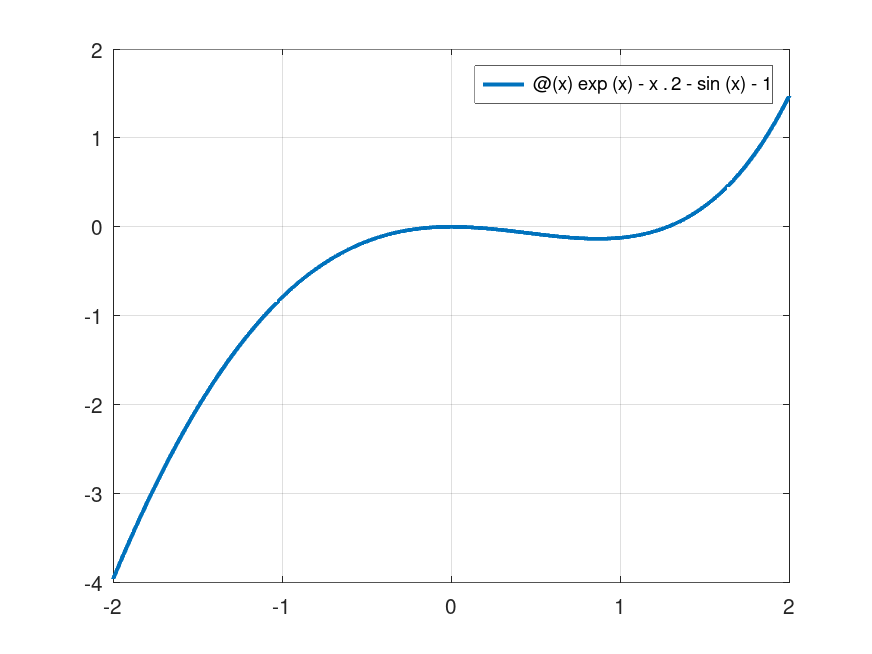
\includegraphics[width=.7\textwidth]{../zeri/graph1.png}
\caption{Grafico di \(f(x) := e^x - x^2 - \sin x - 1\)}
\end{figure}

\begin{esercizio}
Scrivere una funzione
\begin{center}
\lstinline£[c, fc, iter] = bisezione(f, a, b, tol, itmax)£
\end{center}
metodo di bisezione per la ricerca di una funzione \lstinline£f£ nell'intervallo \lstinline£[a, b]£. Qui, \lstinline£tol£ è la tolleranza sull'approssimazione della radice e \lstinline£itmax£ è il numero massimo di iterazioni disposte a fare. Per quanto riguarda l'output, \lstinline£c£ è l'approssimazione trovata, \lstinline£fc£ è \lstinline£f(c)£ e \lstinline£iter£ è il numero di iterazioni fatte effettivamente per arrivare all'approssimazione \lstinline£c£. Testare la funzione per la ricerca di una delle radici di
\[f(x) := e^x - x^2 - \sin x - 1\]
sull'intervallo \([-2, 2]\).
\end{esercizio}

L'implementazione qui sotto usa il {\em teorema degli zeri}\footnote{Sia \(f : [a, b] \to \erre\) continua con \(f(a)f(b) < 0\). Allora esiste \(c \in ]a, b[\) tale che \(f(c) = 0\).} e l'algoritmo di bisezione che descriviamo velocemente.
\begin{enumerate}
\item Iniziamo con \([a_0, b_0] := [a, b]\).
\item Per \(n \in \enne\), consideriamo \([a_n, b_n]\). Se \(f\) si annulla in uno tra i punti \(a_n, b_n, c_n := \frac{a_n+b_n}{2}\), allora qualche zero è stato individuato. Altrimenti, si dà l'intervallo
\[[a_{n+1}, b_{n+1}] := \begin{cases} [a_n, c_n] & \text{se } f(a_n)f(c_n) < 0 \\ [c_n, b_n] & \text{se } f(c_n)f(b_n) > 0 \end{cases}.\]
\end{enumerate}
A tal scopo è utile osservare che per ogni \(c \in [a_n, b_n]\) si ha
\[\lvert c-c_n \rvert \le \frac{b_n - a_n}{2} = \frac{b_0 - a_0}{2^{n+1}} \text{ per ogni } n \in \enne .\]
Questa disuguaglianza dà un stima dell'errore commesso al passo \(n\)-esimo. Ovviamente, per un'implementazione al calcolatore non possiamo procedere indefinitamente: scegliamo di arrestarci quando viene superato un certo limite di iterazioni oppure quando il numero \(\frac{b_n - a_n}{2}\) scende sotto un valore fissato.

\lstinputlisting{../zeri/bisezione.m}

Testiamo il metodo di bisezione su \(f\):

\begin{lstlisting}[numbers=none]
octave> f = @(x) exp(x)-x.^2-sin(x)-1;
octave> [c, fc, iter] = bisezione(f, 1, 1.5, 1e-12, 100)
c = 1.279701331001888
fc = 6.681322162194192e-13
iter = 39
\end{lstlisting}

% *********************************************************************************************

\begin{esercizio}
Scrivere una funzione
\begin{center}
\lstinline£[c, fc, iter] = newton(f, df, x0, tol, itmax)£
\end{center}
che implementa il metodo di \textenglish{Newton-Raphson} per la ricerca di uno zero di una funzione \lstinline£f£ con derivata \lstinline£df£. Qui, \lstinline£x0£ è il punto da cui parte il metodo, \lstinline£tol£ è la tolleranza sull'approssimazione della radice e \lstinline£itmax£ è il numero massimo di iterazioni disposte a fare. Per quanto riguarda l'output, \lstinline£c£ è l'approssimazione trovata, \lstinline£fc£ è \lstinline£f(c)£ e \lstinline£iter£ è il numero di iterazioni fatte effettivamente per arrivare all'approssimazione \lstinline£c£. Testare la funzione per la ricerca di una delle radici di
\[f(x) := e^x - x^2 - \sin x - 1\]
sull'intervallo \([-2, 2]\).
\end{esercizio}

Richiamiamo che il metodo di \textenglish{Newton-Raphson} si scrive come
\[\begin{cases} x_0 \in \erre \text{ scelto} \\ x_{n+1} = x_n - \frac{f(x_n)}{f^\prime (x_n)} \text{ per } n \in \enne \end{cases}\]

Osserviamo che se dobbiamo controllare l'incremento, ci dobbiamo arrestare quando il valore assoluto di \(\frac{f(x_n)}{f^\prime (x_n)}\) scende al di sotto di una certa tolleranza. Anche in questo caso imponiamo un numero massimo di iterazioni. 

\lstinputlisting{../zeri/newton.m}

Testiamo questo metodo su \(f\):

\begin{lstlisting}[numbers=none]
octave> f = @(x) exp(x)-x.^2-sin(x)-1;
octave> df = @(x) exp(x)-2*x-cos(x);
octave> [c, fc, iter] = newton(f, df, 2, 1e-6, 100)
c = 1.279701331001091
fc = 7.083222897108499e-14
iter = 6
\end{lstlisting}

% *********************************************************************************************

\begin{figure}
\centering
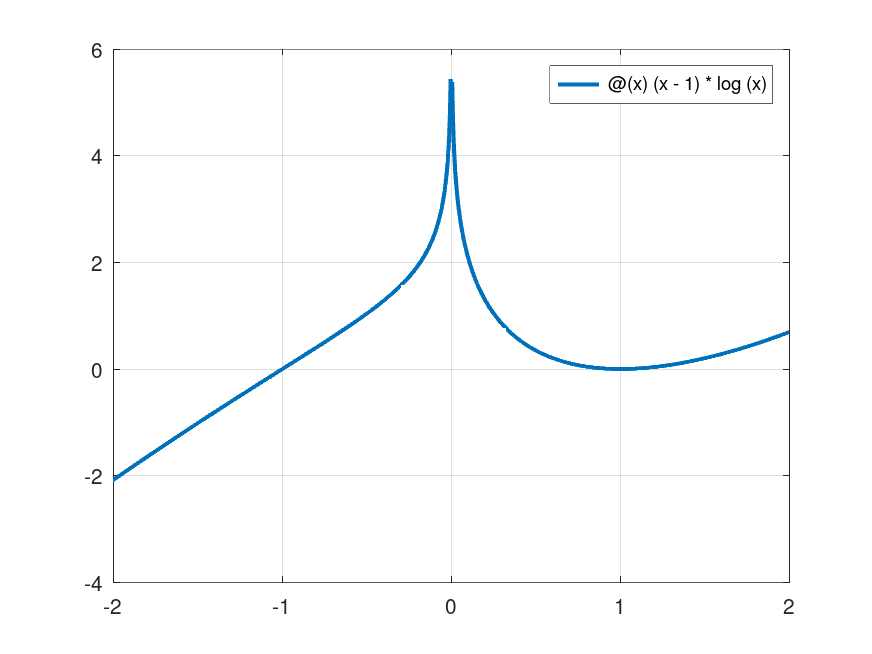
\includegraphics[width=.7\textwidth]{../zeri/graph2.png}
\caption{Grafico di \(f(x) = (x-1)\ln x\)}
\end{figure}

\begin{figure}
\centering
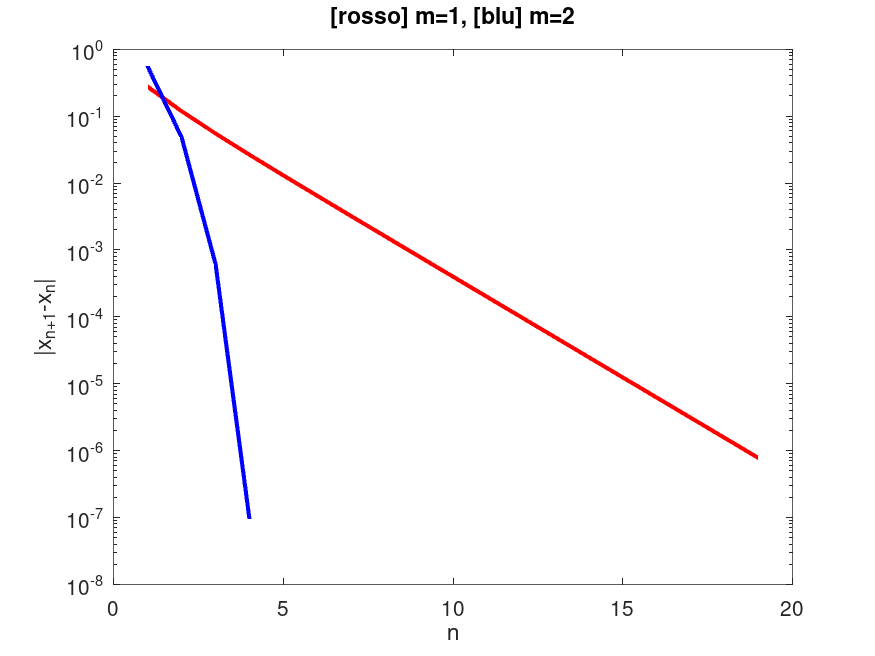
\includegraphics[width=.7\textwidth]{../zeri/convergences.png}
\caption{Grafico degli incrementi al variare del numero di iterazioni}
\label{fig:convergences}
\end{figure}

\begin{esercizio}
Considerare la funzione \(f(x) = (x-1)\ln x\). Applicare il metodo di \textenglish{Newton-Raphson} e il metodo di \textenglish{Newton-Raphson} {\em modificato} per la ricerca della radice doppia \(1\) e confrontare graficamente gli ordini di convergenza dei due metodi.
\end{esercizio}

Se \(\alpha\) è una radice con molteplicità \(m \ge 2\), il metodo di \textenglish{Newton-Raphson} ha ordine \(1\). Se però sappiamo a priori \(m\), possiamo modificare questo metodo così:
\[\begin{cases} x_0 \in \erre \text{ scelto} \\ x_{n+1} = x_n - m\frac{f(x_n)}{f^\prime (x_n)} \text{ per } n \in \enne \end{cases}\]
ed avere una convergenza quadratica.

Modifichiamo \lstinline£newton£ in questo modo: tra gli output teniamo conto di \(m\), c'è un solo output questa volta ed è una lista degli incrementi \(\left\lvert x_{n+1} - x_n \right\rvert\).

\lstinputlisting{../zeri/newton\_errors.m}

Il seguente script disegna il grafico che permette di confrontare la velocità di convergenza nei casi \lstinline£m=1£ e \lstinline£m=2£.

\lstinputlisting{../zeri/convergences.m}
